% Šepet — shema arhitekture (TikZ). Izris: lualatex arhitektura.tex
\documentclass[tikz,border=4pt]{standalone}
\usepackage{fontspec}
\setmainfont{TeX Gyre Heros}[Extension=.otf, UprightFont=texgyreheros-regular, BoldFont=texgyreheros-bold,
  ItalicFont=texgyreheros-italic, BoldItalicFont=texgyreheros-bolditalic]
\usetikzlibrary{positioning,shapes.geometric,arrows.meta,calc,fit,backgrounds}

\definecolor{ink}{HTML}{1F2A37}
\definecolor{muted}{HTML}{6B7280}
\definecolor{svc}{HTML}{2F5E9E}
\definecolor{svcbg}{HTML}{F3F6FB}
\definecolor{dbbg}{HTML}{E6EBF2}
\definecolor{edge}{HTML}{B45F06}
\definecolor{edgebg}{HTML}{FFF6EA}
\definecolor{bus}{HTML}{9C2C5E}
\definecolor{busbg}{HTML}{FBEFF5}
\definecolor{azure}{HTML}{0A6EBD}
\definecolor{azurebg}{HTML}{EAF3FB}
\definecolor{rpc}{HTML}{6B3FA0}
\definecolor{ws}{HTML}{0F7C7E}

\begin{document}
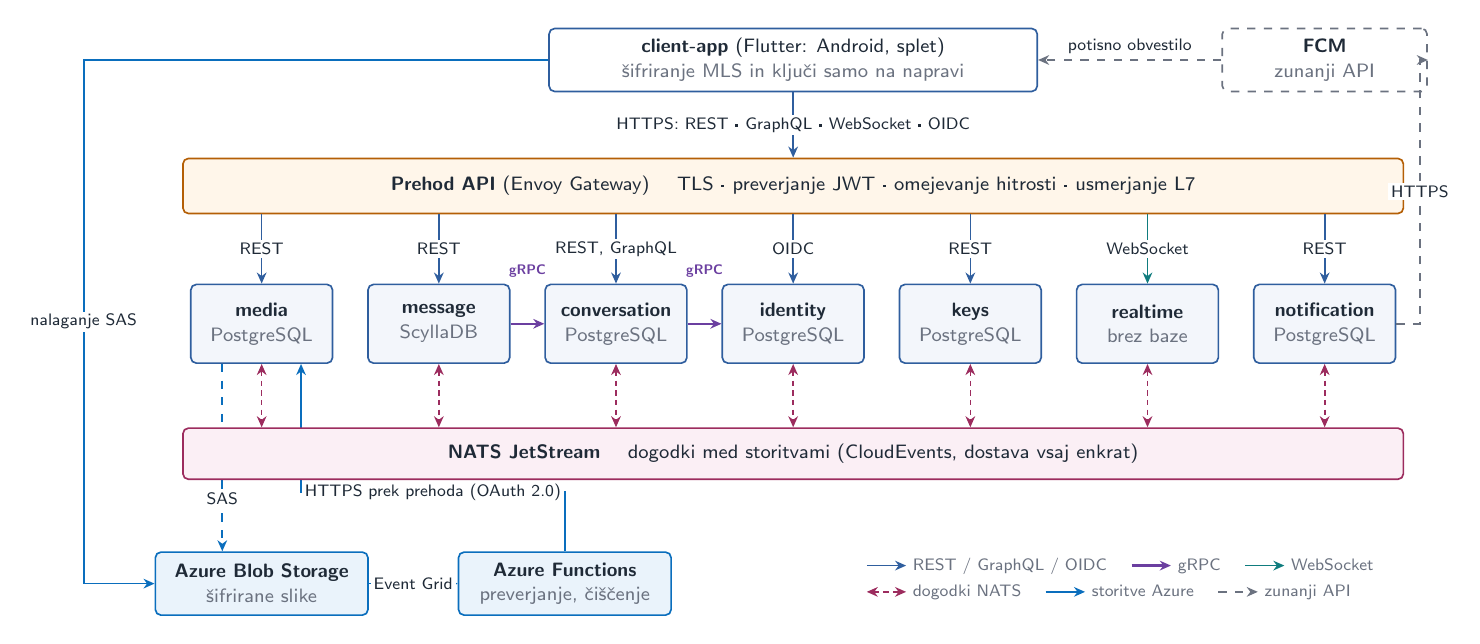
\begin{tikzpicture}[
  font=\sffamily\scriptsize, ink, >={Stealth[length=4pt,width=3.5pt]},
  svc/.style={draw=svc, fill=svcbg, rounded corners=2pt, minimum width=18mm, minimum height=10mm, align=center, line width=0.6pt},
  box/.style={draw=#1, rounded corners=2pt, align=center, line width=0.6pt, inner sep=3pt},
  lbl/.style={fill=white, inner sep=1pt, font=\sffamily\fontsize{6.3}{7.5}\selectfont},
  sync/.style={->, line width=0.6pt, draw=svc},
  evt/.style={<->, line width=0.6pt, draw=bus, dash pattern=on 2pt off 1.5pt},
]
% ---------- storitve (vsaka z lastno bazo) ----------
\def\sx{2.25}
\foreach \i/\n/\db in {0/media/PostgreSQL, 1/message/ScyllaDB, 2/conversation/PostgreSQL, 3/identity/PostgreSQL,
                       4/keys/PostgreSQL, 5/realtime/{brez baze}, 6/notification/PostgreSQL} {
  \node[svc] (s\i) at (1.75+\i*\sx, 0) {\textbf{\n}\\[1pt]{\color{muted}\db}};
}
% ---------- prehod API ----------
\node[box=edge, fill=edgebg, minimum height=7mm, minimum width=155mm] (gw) at (8.5, 1.75)
  {\textbf{Prehod API} (Envoy Gateway) \quad TLS · preverjanje JWT · omejevanje hitrosti · usmerjanje L7};
% ---------- odjemalec in zunanji sistemi ----------
\node[box=svc, fill=white, minimum height=8mm, minimum width=62mm] (app) at (8.5, 3.35)
  {\textbf{client-app} (Flutter: Android, splet)\\[1pt]{\color{muted}šifriranje MLS in ključi samo na napravi}};
\node[box=muted, dashed, fill=white, minimum height=8mm, minimum width=26mm] (fcm) at (15.25, 3.35)
  {\textbf{FCM}\\[1pt]{\color{muted}zunanji API}};
% ---------- NATS ----------
\node[box=bus, fill=busbg, minimum height=6.5mm, minimum width=155mm] (nats) at (8.5, -1.65)
  {\textbf{NATS JetStream} \quad dogodki med storitvami (CloudEvents, dostava vsaj enkrat)};
% ---------- Azure ----------
\node[box=azure, fill=azurebg, minimum height=8mm, minimum width=27mm] (blob) at (1.75, -3.3)
  {\textbf{Azure Blob Storage}\\[1pt]{\color{muted}šifrirane slike}};
\node[box=azure, fill=azurebg, minimum height=8mm, minimum width=27mm] (func) at (5.6, -3.3)
  {\textbf{Azure Functions}\\[1pt]{\color{muted}preverjanje, čiščenje}};

% ---------- povezave: odjemalec ----------
\draw[sync, line width=0.9pt] (app.south) -- node[lbl]{HTTPS: REST · GraphQL · WebSocket · OIDC} (gw.north -| app.south);
\draw[->, line width=0.6pt, draw=muted, dashed] (fcm.west) -- node[lbl, above=1pt, fill=none]{potisno obvestilo} (app.east);
\draw[->, line width=0.6pt, draw=azure] (app.west) -- ++(-5.9,0) |- node[lbl, pos=0.25]{nalaganje SAS} (blob.west);

% ---------- povezave: prehod -> storitve ----------
\foreach \i/\p in {0/REST, 1/REST, 2/{REST, GraphQL}, 3/OIDC, 4/REST, 6/REST} {
  \draw[sync] (gw.south -| s\i.north) -- node[lbl]{\p} (s\i.north);
}
\draw[->, line width=0.6pt, draw=ws] (gw.south -| s5.north) -- node[lbl]{WebSocket} (s5.north);

% ---------- gRPC ----------
\draw[->, line width=0.8pt, draw=rpc] (s1.east) -- (s2.west);
\draw[->, line width=0.8pt, draw=rpc] (s2.east) -- (s3.west);
\node[font=\sffamily\tiny\bfseries, text=rpc] at ($(s1.north east)!0.5!(s2.north west)+(0,0.16)$) {gRPC};
\node[font=\sffamily\tiny\bfseries, text=rpc] at ($(s2.north east)!0.5!(s3.north west)+(0,0.16)$) {gRPC};

% ---------- dogodki ----------
\foreach \i in {0,1,2,3,4,5,6} { \draw[evt] (s\i.south) -- (s\i.south |- nats.north); }

% ---------- Azure ----------
\begin{pgfonlayer}{background}
\draw[->, line width=0.6pt, draw=azure, dashed] ([xshift=-5mm]s0.south) -- node[lbl, pos=0.72]{SAS} ([xshift=-5mm]s0.south |- blob.north);
\draw[->, line width=0.6pt, draw=azure] (blob.east) -- node[lbl]{Event Grid} (func.west);
\draw[->, line width=0.6pt, draw=azure] (func.north) -- ++(0,0.75) -| node[lbl, pos=0.25]{HTTPS prek prehoda (OAuth 2.0)} ([xshift=5mm]s0.south);
\end{pgfonlayer}
\draw[->, line width=0.6pt, draw=muted, dashed] (s6.east) -- ++(0.3,0) |- node[lbl, pos=0.25]{HTTPS} (fcm.east);

% ---------- legenda ----------
\node[anchor=north west, align=left, font=\sffamily\fontsize{6.3}{7.5}\selectfont, text=muted] at (9.3, -2.85) {%
  \tikz{\draw[->, svc, line width=0.6pt] (0,0) -- (0.5,0);} REST / GraphQL / OIDC \quad
  \tikz{\draw[->, rpc, line width=0.8pt] (0,0) -- (0.5,0);} gRPC \quad
  \tikz{\draw[->, ws, line width=0.6pt] (0,0) -- (0.5,0);} WebSocket\\[2pt]
  \tikz{\draw[<->, bus, line width=0.6pt, dash pattern=on 2pt off 1.5pt] (0,0) -- (0.5,0);} dogodki NATS \quad
  \tikz{\draw[->, azure, line width=0.6pt] (0,0) -- (0.5,0);} storitve Azure \quad
  \tikz{\draw[->, muted, dashed, line width=0.6pt] (0,0) -- (0.5,0);} zunanji API};
\end{tikzpicture}
\end{document}
